%----------------------------------------------------------------------------------------
%
% A LaTeX-template for 1DV510. Modified and translated by Björn Lindenberg at LNU.
% Based on an original master thesis template created by Marcus Wilhelmsson at LNU.
%
%----------------------------------------------------------------------------------------

% Settings and document configuration

\documentclass[a4paper,12pt]{article} 
\usepackage[T1]{fontenc} 
\usepackage{times} 
\usepackage[swedish,english]{babel} 
\usepackage[utf8]{inputenc} 
\usepackage{dtk-logos} 
\usepackage{wallpaper} 
\usepackage[absolute]{textpos} 
\usepackage[top=2cm, bottom=2.5cm, left=3cm, right=3cm]{geometry} 
\usepackage[parfill]{parskip} 
\usepackage{csquotes} 
\usepackage{float} 
\usepackage{lipsum} % Used for dummy text. Can be removed.
\usepackage{amsmath}
\usepackage{multirow}
\usepackage{tikz}
% Fontsizes for section headings.
\usepackage{sectsty} 

\sectionfont{\fontsize{14}{15}\selectfont}
\subsectionfont{\fontsize{12}{15}\selectfont}
\subsubsectionfont{\fontsize{12}{15}\selectfont}

%----------------------------------------------------------------------------------------
%	This part is used for the text box on the title page
%----------------------------------------------------------------------------------------
\newsavebox{\mybox}
\newlength{\mydepth}
\newlength{\myheight}

\newenvironment{sidebar}%
{\begin{lrbox}{\mybox}\begin{minipage}{\textwidth}}%
{\end{minipage}\end{lrbox}%
 \settodepth{\mydepth}{\usebox{\mybox}}%
 \settoheight{\myheight}{\usebox{\mybox}}%
 \addtolength{\myheight}{\mydepth}%
 \noindent\makebox[0pt]{\hspace{-20pt}\rule[-\mydepth]{1pt}{\myheight}}%
 \usebox{\mybox}}

%----------------------------------------------------------------------------------------
%	Title
%----------------------------------------------------------------------------------------
\newcommand\BackgroundPic{
    \put(-2,-3){
    \includegraphics[keepaspectratio,scale=0.3]{img/lnu_etch.png} % Background image
    }
}
\newcommand\BackgroundPicLogo{
    \put(30,740){
    \includegraphics[keepaspectratio,scale=0.10]{img/logo.png} % LNU logo
    }
}

\title{
\vspace{-8cm}
\begin{sidebar}
    \vspace{10cm}
    \normalfont \normalsize
    \huge \LaTeX{} Introduction\\ % Main title
    \vspace{-1.3cm}
\end{sidebar}
\vspace{3cm}
\begin{flushleft}
    \huge Template for your report % Subtitle
\end{flushleft}
\null
\vfill
\begin{textblock}{5}(10,13)
\begin{flushright}
\begin{minipage}{\textwidth}
\begin{flushleft} \large
\emph{Authors:} Daniel \textsc{Holmkvist}, Rasmus \textsc{Svensson}\\  % Author
\emph{Semester:} HT2017\\ % Semester
\emph{Area:} Computer Science \\ % Area
\emph{Course code:} 1DV510 % Course
\end{flushleft}
\end{minipage}
\end{flushright}
\end{textblock}
}

\date{} % Empty date command. Use \today inside for today's date.
\author{} % Normally one would use this to define authors. However in this case the title command takes care of everything, so we leave the field empty to get rid of warnings. 

\begin{document}

\pagenumbering{gobble} % Turn off page numbering
\newgeometry{left=5cm}
\AddToShipoutPicture*{\BackgroundPic} % Adds the background image to the title page
\AddToShipoutPicture*{\BackgroundPicLogo} % Adds the logo to the title page
\maketitle % Prints the title
\restoregeometry
\clearpage

\pagenumbering{roman} % Roman page numbering for abstract page
\selectlanguage{swedish}

\begin{abstract}
\noindent Swedish abstract.
\end{abstract}

\selectlanguage{english}
\begin{abstract}
\noindent English abstract.

\end{abstract}

\selectlanguage{swedish}

\newpage

\pagenumbering{gobble} % Turn off page numbering
\tableofcontents 

\newpage
\pagenumbering{arabic} % Turn on page numbering

% Some example sections with dummy text
\section{Assignments}
\subsection{Assignment 1}
\fontfamily{cmr}\selectfont
Den här texten använder Computer Modern Roman.  \\
\fontfamily{ptm}\selectfont
Denna använder times.
\subsection{Assignment 2}
\begin{equation*}
	\frac{\sin mx}{\sin x} = (-4)^{(m-1)/2} \prod_{j=1}^{(m-1)/2} 
	\left( \sin^2x - sin^2\frac{2\pi j}{m} \right)
\end{equation*}
Ekvationer kan också skrivas inline $f_n = f_{n-1} + f_{n-2} $ likt här.
\subsection{Assignment 3 \& 4}
Som kan ses av tabell \ref{tab:records} är Anna-Karin... 
\begin{table}[htbp]
	\centering
	\begin{tabular}{c c c c}
		\hline 
		& & \multicolumn{2}{c}{\textbf{World Record}} \\ \cline{3-4}
		\bfseries{Name} & \bfseries{Country} & \bfseries{Event} & 				\bfseries{Result} \\ 
		\hline 
		Anna-Karin Kammerling & Sweden & 50 m butterfly & 25.57 \\ 
		Wilson Kipketer & Denmark & 800 m & 2:11.96 \\ 
		Jan \v{Z}elezný & Czech Republic & javelin throw & 98.5 \\ 
		Sergei Bubka & Ukraine & pole vault & 6.14 \\ 
		\hline 
	\end{tabular} 
	\caption{Tabellen visar}
	\label{tab:records}
\end{table}
\subsection{Assignment 5}
Som kan ses av figur \ref{f:tikz} ...
\begin{figure}[htbp]
	\centering
	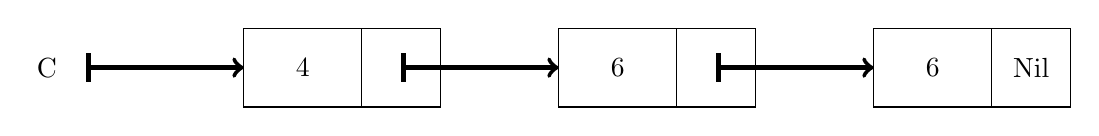
\begin{tikzpicture}
		\node at (0.5,0) {C};
		\draw [|->, ultra thick] (1,0) -- (3,0);
		\node at (3.75,0) {4};
		\draw (3,-0.5) rectangle (4.5,0.5);
		\draw (4.5,-0.5) rectangle (5.5,0.5);
		\draw [|->, ultra thick] (5,0) -- (7,0);
		\node at (7.75,0) {6};
		\draw (7,-0.5) rectangle (8.5,0.5);
		\draw (8.5,-0.5) rectangle (9.5,0.5);
		\draw [|->, ultra thick] (9,0) -- (11,0);
		\node at (11.75,0) {6};
		\draw (11,-0.5) rectangle (12.5,0.5);
		\draw (12.5,-0.5) rectangle (13.5,0.5);
		\node at (13,0) {Nil};
	\end{tikzpicture}
	\caption{Här är en TikZ bild }
	\label{f:tikz}
\end{figure}
\subsection{Assignment 6}
I figur \ref{f:bild} ...
\begin{figure}[htbp]
	\centering
	\includegraphics[scale=0.65]{img/binaryimpl}
	\caption{Här är en infogad bild}
	\label{f:bild}
\end{figure}
\subsection{Assignment 8}
(a) I a krävs användandet av klammerparenteser, vilka måste även avslutas. Då kan koden se ut på följande sätt:
 $x^{n^2} + y^{n + 1} = z^n $ I
(b) \textbackslash emph skrivs med enbart ett 'h'. Och tecken (\&) måste skrivas med ett backslash före då det har betydelse för kommandon i \LaTeX . 
\begin{center}
	\emph{The Johansson Brothers \& Son}
\end{center}
(c) .. end of a paragraph. 

A new paragraph ... 
\section{Methods}
\section{Results}
\section{Discussion}
H. Jass proved in \cite{big} that\ldots \ Therefore, as stated in \cite{Creswell2014}, $e = m c^2$.

% Prints your bibliography database xxx.bib
\bibliographystyle{IEEEtran}
\bibliography{ref.bib}

\end{document}
